\documentclass[12pt]{article}
\usepackage{latexsym,amssymb,amsmath} % for \Box, \mathbb, split, etc.
% \usepackage[]{showkeys} % shows label names
\usepackage{cite} % sorts citation numbers appropriately
\usepackage{path}
\usepackage{url}
\usepackage{verbatim}
\usepackage[pdftex]{graphicx}

% horizontal margins: 1.0 + 6.5 + 1.0 = 8.5
\setlength{\oddsidemargin}{0.0in}
\setlength{\textwidth}{6.5in}
% vertical margins: 1.0 + 9.0 + 1.0 = 11.0
\setlength{\topmargin}{0.0in}
\setlength{\headheight}{12pt}
\setlength{\headsep}{13pt}
\setlength{\textheight}{625pt}
\setlength{\footskip}{24pt}

\renewcommand{\textfraction}{0.10}
\renewcommand{\topfraction}{0.85}
\renewcommand{\bottomfraction}{0.85}
\renewcommand{\floatpagefraction}{0.90}

\makeatletter
\setlength{\arraycolsep}{2\p@} % make spaces around "=" in eqnarray smaller
\makeatother

% change equation, table, figure numbers to be counted inside a section:
\numberwithin{equation}{section}
\numberwithin{table}{section}
\numberwithin{figure}{section}

% begin of personal macros
\newcommand{\half}{{\textstyle \frac{1}{2}}}
\newcommand{\eps}{\varepsilon}
\newcommand{\myth}{\vartheta}
\newcommand{\myphi}{\varphi}

\newcommand{\IN}{\mathbb{N}}
\newcommand{\IZ}{\mathbb{Z}}
\newcommand{\IQ}{\mathbb{Q}}
\newcommand{\IR}{\mathbb{R}}
\newcommand{\IC}{\mathbb{C}}
\newcommand{\Real}[1]{\mathrm{Re}\left({#1}\right)}
\newcommand{\Imag}[1]{\mathrm{Im}\left({#1}\right)}

\newcommand{\norm}[2]{\|{#1}\|_{{}_{#2}}}
\newcommand{\abs}[1]{\left|{#1}\right|}
\newcommand{\ip}[2]{\left\langle {#1}, {#2} \right\rangle}
\newcommand{\der}[2]{\frac{\partial {#1}}{\partial {#2}}}
\newcommand{\dder}[2]{\frac{\partial^2 {#1}}{\partial {#2}^2}}
\usepackage{enumitem}
\newcommand{\nn}{\mathbf{n}}
\newcommand{\xx}{\mathbf{x}}
\newcommand{\uu}{\mathbf{u}}
\usepackage{tikz}
\usetikzlibrary{arrows}
\usetikzlibrary{positioning}
\usepackage{titlesec}
\newcommand{\junk}[1]{{}}
\usepackage{sectsty}
\usepackage{xcolor}

\makeatletter
\renewcommand*\env@matrix[1][\arraystretch]{%
	\edef\arraystretch{#1}%
	\hskip -\arraycolsep
	\let\@ifnextchar\new@ifnextchar
	\array{*\c@MaxMatrixCols c}}
\makeatother

\makeatletter
\renewcommand*\env@matrix[1][*\c@MaxMatrixCols c]{%
	\hskip -\arraycolsep
	\let\@ifnextchar\new@ifnextchar
	\array{#1}}
\makeatother

\definecolor{darkblue}{rgb}{0,0,0.4}
\usepackage[colorlinks = true,
linkcolor = darkblue,
urlcolor  = darkblue,
citecolor = darkblue,
anchorcolor = darkblue]{hyperref}
% set two lengths for the includegraphics commands used to import the plots:
\newlength{\fwtwo} \setlength{\fwtwo}{0.45\textwidth}
% end of personal macros

\begin{document}
\DeclareGraphicsExtensions{.jpg}

\begin{center}
\textsc{\Large Multi-core Programming} \\[2pt]
	\textsc{\large Assignment 1}\\
	\vspace{0.5cm}
  Ali Gholami \\[6pt]
  Department of Computer Engineering \& Information Technology\\
  Amirkabir University of Technology  \\[6pt]
  \def\UrlFont{\em}
  \url{http://ceit.aut.ac.ir/~aligholamee}\\
    \href{mailto:aligholamee@aut.ac.ir}{\textit{aligholamee@aut.ac.ir}}
\end{center}

\begin{abstract}
This assignment reviews principal architectures for a parallel computer. Two main architectures as \textit{Shared Memory} and \textit{Message Passing} and their subtypes like \textit{UMA, NUMA, hUMA} and \textit{COMA} are introduced. We'll also review the substantial \textit{Amdahl's law}, \textit{Gustafson Barsis's law} and \textit{Sun-Ni’s law} to understand the \textit{performance} and \textit{scalability} of parallel architectures. Finally, we'll be measuring various metrics for parallelism in an \textit{Asus N56JK} laptop.
\end{abstract}

\subparagraph{Keywords.} \textit{Parallel Architecture, Multi-core, Multi-thread, Uniform Memory Access, NUMA, COMA, Amdahl, Gustafson Barsis, Sun-Nis.}

\section{Communication Models in Parallel Computers}
There are different communication models in parallel computers. The two main architectures are \textit{Shared Memory} and \textit{Message Passing}.
\subsection*{Shared Memory}
In a computer with \textit{shared memory} architecture among its processors, each of its processors can access the memory simultaneously with other processors. The intuition can be represented as figure 1.1.
\begin{figure}[!h]\centering
	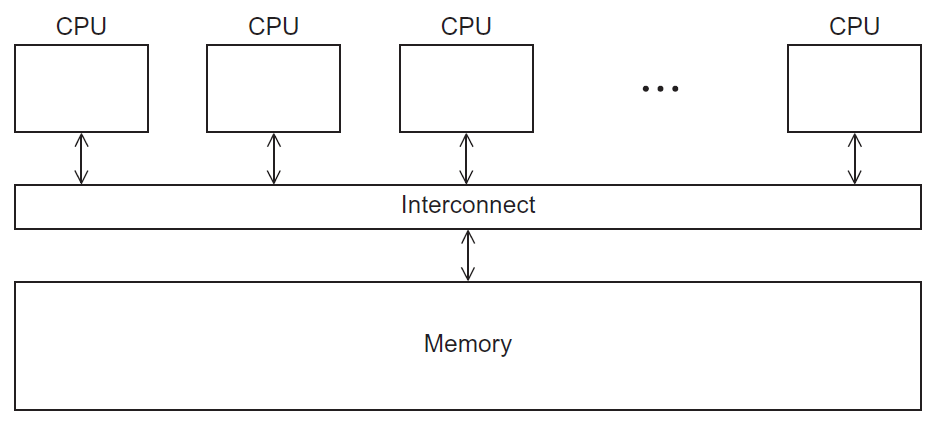
\includegraphics[width=0.6\textwidth]{Shared_memory_1.png}
	\caption{A simple shared memory architecture with multiple processors.}
	\label{figsolplot}
\end{figure}\\
A shared memory architecture conducts two main physical architectures:
\begin{itemize}
	\item Non-distributed Shared Memory
	\item Distributed Shared Memory
\end{itemize}
A \textit{Non-distributed Shared Memory} was introduced in figure 1.1. As a physical point of view, the \textit{Non-distributed Shared Memory} is \textit{centralized} memory that can be accessed by the processors through a \textit{communication bus}.
Memories can be physically independent of each other. They can be implemented with processors. In this case, each processors has its own memory which is called a \textit{Distributed Shared Memory}. An intuition of this architecture can be grasped by looking at figure 1.2.
\begin{figure}[!h]\centering
	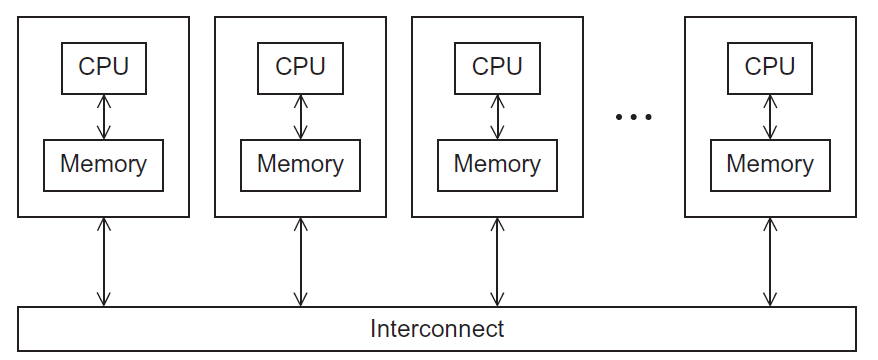
\includegraphics[width=0.6\textwidth]{Shared_memory_2.png}
	\caption{A distributed shared memory architecture with multiple processors.}
	\label{figsolplot}
\end{figure}\\
Accessing the memory can be either \textit{uniform} or \textit{non-uniform}. We'll describe each further.
\subsection*{UMA}
\begin{figure}[!h]\centering
	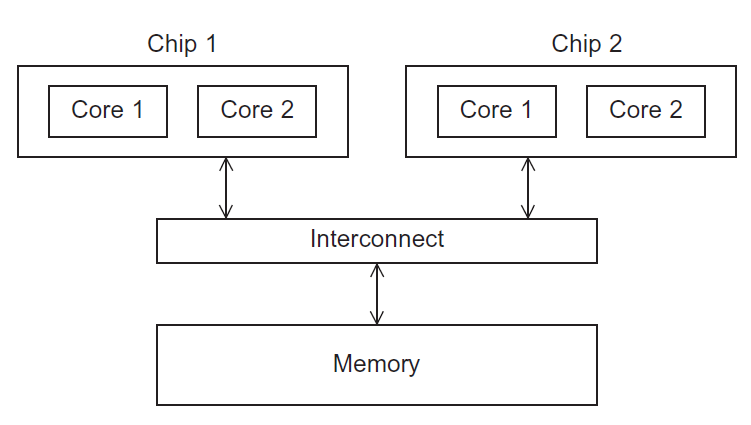
\includegraphics[width=0.6\textwidth]{UMA_1.png}
	\caption{Demonstration of Uniform Memory Access in Shared Memory Architecture.}
	\label{figsolplot}
\end{figure}
\textit{UMA} stands for \textit{Uniform Memory Access}. This is called \textit{uniform} because, each of the processors have the same \textit{Access Time} to the memory. Some of the features for \textit{UMA} is given below:
\begin{enumerate}
	\item Suitable for \textit{Time Sharing} applications by multiple users.
	\item It can be used to speed up a single large program in a \textit{Time Critical} application.
\end{enumerate}
\subsection*{NUMA}
\begin{figure}[!h]\centering
	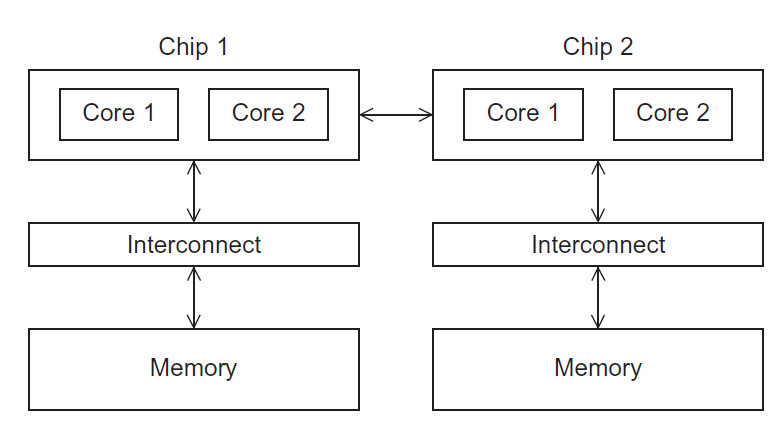
\includegraphics[width=0.6\textwidth]{NUMA_1.png}
	\caption{Demonstration of Non-uniform Memory Access in Shared Memory Architecture.}
	\label{figsolplot}
\end{figure}
\textit{NUMA} Stands for \textit{Non-uniform Memory Access}. The \textit{Memory Access Time} could be different for each processor. To be more accurate, \textit{NUMA} is the phenomenon that memory at various points in the address space of a processor have different performance characteristics. A \textit{NUMA} system classifies memory into \textit{NUMA} nodes. All memory available in one node has the same access characteristics for a particular processor. Nodes have an affinity to processors and to devices. These are the devices that can use memory on a \textit{NUMA} node with the best performance since they are locally attached.\cite{NUMA}

\subsection*{hUMA}
In 2013, \textit{AMD} introduced \textit{hUMA}; \textit{heterogeneous Unifrom Memory Access}. Before that, \textit{AMD} had talked about the \textit{HSA} concept which stands for \textit{Heterogeneous Systems Architecture}. This concepts depicts that systems could have multiple different kinds of processors. More specifically, \textit{versatile CPUs} and \textit{specialized GPUs} can be integrated on a system. Let's dive into the history and find the root of this invention.
\begin{enumerate}
	\item	Modern \textit{GPUs} have enormous parallel arithmetic power, especially floating point arithmetic, but are poorly-suited to \textit{single-threaded} code with lots of branches.
	\item Modern \textit{CPUs} are well-suited to \textit{single-threaded} code with lots of branches, but less well-suited to massively parallel number crunching.
\end{enumerate}
Thus, Splitting workloads between a \textit{CPU} and a \textit{GPU}, using each for the workloads it's good at, has driven the development of general purpose \textit{GPU (GPGPU)} software and development.\newpage
But there still exists some problems:
\begin{enumerate}
	\item The \textit{CPU} and \textit{GPU} have their own pools of memory. Physically, these might use the same chips on the motherboard (as most integrated \textit{GPUs} carve off a portion of system memory for their own purposes). From a software perspective, however, these are completely separate.
	\item This means that whenever a CPU program wants to do some computation on the \textit{GPU}, it has to copy all the data from the \textit{CPU's} memory into the \textit{GPU's} memory. When the \textit{GPU} computation is finished, all the data has to be copied back. This need to copy back and forth wastes time and makes it difficult to mix and match code that runs on the \textit{CPU} and code that runs on the GPU.
\end{enumerate}
\subsubsection*{AMD's Magic}
With \textit{hUMA}, the \textit{CPU} and \textit{GPU} share a \underline{single memory space}. The \textit{GPU} can directly access \textit{CPU} memory addresses, allowing it to \underline{both read and write data} that the \textit{CPU} is also reading and writing.
\subsubsection*{Cache-coherent vs Non-cache-coherent Systems}
hUMA is a cache coherent system.
\begin{itemize}
	\item In \textit{non-cache-coherent} systems, programs have to explicitly signal that they have changed data that other processors might have cached, so that those other processors can discard their stale cached copy. This \underline{makes the hardware simpler}, but introduces great scope for \underline{software errors} that result in bugs that are hard to detect, diagnose, and fix.
	
	\item
	In a \textit{cache-coherent} the \textit{CPU} and \textit{GPU} will always see a consistent view of data in memory. If one processor makes a change then the other processor will see that changed data, even if the old value was being cached.\cite{hUMA}
\end{itemize}

\subsection*{COMA}
The shared memory concept makes it easier to write parallel programs, but tuning the application to reduce the impact of frequent long latency memory accesses still requires substantial programmer effort. Researchers have proposed using compilers, operating systems, or architectures to improve performance by allocating data close to the processors that use it. The Cache-Only Memory Architecture (\textit{COMA}) \underline{increases the chances} of data being available locally because \underline{the hardware transparently replicates the data and migrates it to the memory} module of the node that is currently accessing it. Each memory module acts as a huge cache memory in which each block has a tag with the address and the state.\cite{COMA}
In NUMA, each address in the global address space is typically assigned a fixed home node. When processors access some data, a copy is made in their local cache, but space remains allocated in the home node. Instead, with COMA, there is no home. An access from a remote node may cause that data to migrate.
\begin{itemize}
	\item It reduces the number of redundant copies and may allow more efficient use of the memory resources.
	
	\item It raises problems of how to find a particular data (there is no longer a home node) and what to do if a local memory fills up.
\end{itemize}
\begin{thebibliography}{9}
	\bibitem{NUMA} 
	Christoph Lameter. 
	\textit{NUMA (Non-Uniform Memory Access): An Overview}. ACM Queue, Vol. 11, no. 7. Retrieved on September 1st, 2015.
	
	\bibitem{hUMA} 
	Peter Bright. 
	\textit{AMD's "heterogeneous Uniform Memory Access" coming this year in Kaveri}. Ars Technica, April 30, 2013.
	
	\bibitem{COMA} 
	F. Dahlgren and J. Torrellas. 
	\textit{Cache-only memory architectures}. IEEE Computer, June 1999.
\end{thebibliography}

\end{document}